
\section{维数与余维}

\textbf{12.1.1.}\ \emph{\trhDefinition{}（们）：\trDimension{}。}\quad 出人意料的是，正确的定义竟是纯拓扑的——它只依赖于\trTopologicalSpace{}本身，而不依赖于\trStructureSheaf。我们把\trTopologicalSpace{} $X$ 的\textbf{\trDimension}（记作 $\dim X$）定义为诸\trIrreducible{}\trClosedSet{}之链的长度的上确界，其中诸不可约闭集自 $0$ 起编号。（\trDimension{}可以是无穷的。）研究空集的学者不妨把空集的\trDimension{}取作 $-\infty$。（一个来自线性代数的类比：\trVectorSpace{}的\trDimension{}是诸子空间之链的长度的上确界。）把一个\trRing{}的\trDimension{}定义为诸嵌套\trPrimeIdeal{}之链的长度的上确界（编号自零起）。\trDimension{}的这两版定义有时被称为\textbf{\trKrullDimension}（Krull dimension）。（你也许会认为\trNoetherian{}环必具有有限的\trDimension{}，因为\trPrimeIdeal{}的链都是有限的——但这并不必然成立，见\mbox{练习~12.1.M}。）

\textbf{12.1.A.（容易的练习）}\quad 证明：$\dim\Spec A=\dim A$。（提示：\cref{ex:irreducible-prime-bijection}给出了 $\Spec A$ 的诸\trIrreducible{}\trClosedSubset{}与 $A$ 的诸\trPrimeIdeal{}之间的一个双射。这个双射是「反转包含关系」的。）

$\Spec A$ 与 $\Spec A/\mathfrak{N}(A)$ 之间的\trHomeomorphism{}（\S3.4.7：\trZariskiTopology{}不理会\trNilpotent{}元）蕴涵 $\dim\Spec A=\dim\Spec A/\mathfrak{N}(A)$。

\textbf{12.1.2.}\ \emph{\trhExample{}。}\quad 我们已经辨认出 $k[t]$ 的全部\trPrimeIdeal{}（它们是 $0$，以及对\trIrreducible{}多项式 $f(t)$ 的 $(f(t))$）、$\mathbb{Z}$ 的全部\trPrimeIdeal{}（$(0)$ 与诸 $(p)$）、$k$ 的全部\trPrimeIdeal{}（只有 $(0)$），以及 $k[x]/(x^2)$ 的全部\trPrimeIdeal{}（只有 $(x)$），于是可以迅速核验：$\dim\mathbb{A}^1_k=\dim\Spec\mathbb{Z}=1$，$\dim\Spec k=0$，$\dim\Spec k[x]/(x^2)=0$。

\textbf{12.1.3.}\quad 对可约空间而言，\trDimension{}这个观念必须小心对待。若 $Z$ 是两个\trClosedSubset{} $X$ 与 $Y$ 的并，则 $\dim Z=\max(\dim X,\dim Y)$。从而\trDimension{}并不是一个空间的「局部」特征。这件事有时令我们困扰，所以我们尽量只谈\trIrreducible{}\trTopologicalSpace{}的\trDimension。我们说一个\trTopologicalSpace{}是\textbf{\trPureDimensional{}的}（pure dimensional）或\textbf{\trEquidimensional{}的}（equidimensional）（相应地，具有\textbf{\trPureDimension{} $n$}（pure dimension $n$）或\textbf{维数为 $n$ 的\trEquidimensional}（equidimensional of dimension $n$）），若它的每个\trIrreducibleComponent{}都具有相同的\trDimension（相应地，它们全都具有\trDimension{} $n$）。\trPureDimension{} $1$（相应地，$2$、$n$）的\trTopologicalSpace{}称为一条\textbf{\trCurve}（相应地，一张\textbf{\trSurface}、一个\textbf{\trNFold}（$n$-fold））。

\textbf{12.1.B.（有用的练习）}\quad 证明：一个\trScheme{}的\trDimension{}为 $n$，当且仅当它有一个由\trDimension{}至多为 $n$ 的\trAffine\trOpenSubset{}构成的\trOpenCover，并且等号在其中某个\trAffine\trOpenSubset{}上达到。提示：你或许会发现，证明下面这件事在此处和日后都有帮助。对任意\trTopologicalSpace{} $X$ 与\trOpenSubset{} $U\subset X$，$U$ 的诸\trIrreducible{}\trClosedSubset{}与 $X$ 的同 $U$ 相交的诸\trIrreducible{}\trClosedSubset{}之间存在一个双射。

\textbf{12.1.C.（容易的练习）}\quad 证明：\trDimension{}为 $0$ 的\trNoetherian\trScheme{}只有有限多个点。

\textbf{12.1.D.（容易的练习）}\quad 证明：具有同一有限\trDimension{}的诸\trIntegralDomain{}之间的\trSurjectiveMap{}必是\trIsomorphism。

\textbf{12.1.E.（练习：\trIntegral{}态射的纤维；\S8.3.8 中所许诺的）}\quad 设 $\pi\colon X\to Y$ 是一个\trIntegral{}态射。证明：$\pi$ 的每个（非空）\trFiber{}的\trDimension{}都是 $0$。提示：由于\trIntegral{}态射对\trBaseChange{}保持（\mbox{练习~10.4.D(d)}），我们可以假设 $Y=\Spec k$。于是要证的就是：若 $\phi\colon k\to A$ 是一个\trIntegralExtension，则 $\dim A=0$。证明概要：设 $\mathfrak{p}\subset\mathfrak{m}$ 是 $A$ 的两个\trPrimeIdeal。对 $\mathfrak{p}$ 取商，便可假设 $A$ 是\trIntegralDomain。我断言：任何非零元素都是\trInvertible{}的。比如说 $x\in A$ 且 $x\neq0$。那么 $x$ 的\trMinimalPolynomial（首一的）具有非零常数项。但这样一来 $x$ 就\trInvertible{}了——回想这些系数位于一个\trField{}之中。

\textbf{12.1.F.（重要练习）}\quad 证明：若 $\pi\colon\Spec A\to\Spec B$ 相应于诸\trRing{}的一个\trIntegralExtension，则 $\dim\Spec A=\dim\Spec B$。提示：证明「楼下」的一条\trPrimeIdeal{}链借 Going-Up 定理（\cref{ex:going-up-theorem}）给出「楼上」的一条等长的链。反过来，「楼上」的一条链给出「楼下」的一条链。用\mbox{练习~12.1.E}证明：「楼上」这条链的任何两个元素都不会被送到「楼下」这条链的同一个元素 $[\mathfrak{q}]\in\Spec B$ 上。

\textbf{12.1.G.（练习）}\quad 证明：若 $\nu\colon\widetilde{X}\to X$ 是一个\trScheme{}的\trNormalization（可能是在 $X$ 的\trFunctionField{}的某个\trFiniteFieldExtension{}中取的），则 $\dim\widetilde{X}=\dim X$。为方便起见，你尽管假设 $X$ 是\trIntegral{}的。

\textbf{12.1.H.（有用的练习）}\quad 设 $X$ 是一个仿射 $k$-\trScheme，而 $K/k$ 是一个\trAlgebraic\trFieldExtension。
\begin{enumerate}[label=(\alph*)]
\item 设 $X$ 具有\trPureDimension{} $n$。证明：$X_K:=X\times_k K$ 具有\trPureDimension{} $n$。（一个推广见\mbox{练习~24.5.F}，它比方说去掉了仿射假设。向任意\trFieldExtension{}的种种可能推广的命运如何，另见\mbox{练习~12.2.M}与注记~12.2.17。）提示：若 $X=\Spec A$，化归到 $A$ 是\trIntegralDomain{}的情形。$X_K$ 的一个\trIrreducibleComponent{}对应于 $A_K:=A\otimes_k K$ 的一个\trMinimalPrime{} $\mathfrak{p}$。设 $a\in\ker(A\to A_K/\mathfrak{p})$。利用下面两件事证明 $a=0$：$a$ 落在 $A_K$ 的一个\trMinimalPrime{} $\mathfrak{p}$ 中（从而由 \S6.6.23 它是\trZerodivisor），并且 $A_K$ 是一个自由 $A$-\trModule（于是只要 $a\in A$ 非零，在 $A_K$ 中用 $a$ 相乘就是单的）。这样便知 $A\to A_K/\mathfrak{p}$ 是单的。随后用\mbox{练习~12.1.F}。
\item 证明 (a) 的逆命题：证明：若 $X_K$ 具有\trPureDimension{} $n$，则 $X$ 具有\trPureDimension{} $n$。
\end{enumerate}

\textbf{12.1.I.（练习）}\quad 证明：$\dim\mathbb{Z}[x]=2$。（提示：$\mathbb{Z}[x]$ 的诸\trPrimeIdeal{}曾在\cref{ex:affine-space-over-z-picture}中被隐含地确定过。）

\textbf{12.1.4.\ \trCodimension。}\quad 由于\trDimension{}在\trDisjointUnion{}之下表现古怪，我们在定义\trCodimension{}以及使用这个词时都需要一些小心。例如，若 $Y$ 是 $X$ 的一个\trClosedSubset，我们或许会把\trCodimension{}定义为 $\dim X-\dim Y$，但这种定义表现很糟。比如说，若 $X$ 是一个点 $Y$ 与一条\trCurve{} $Z$ 的\trDisjointUnion，则 $\dim X-\dim Y=1$，但这同 $X$ 在 $Y$ 附近的局部行为毫无关系。

更好的定义如下。为了避免过多的病理，我们\emph{只}在 $Y$ \trIrreducible{}时才定义 $Y$ 在 $X$ 中的\trCodimension。（在任何别的场合使用这个词时，务必要极端小心。）\trTopologicalSpace{}的\trIrreducible{}子集 $Y\subset X$ 的\textbf{\trCodimension}{}定义为：以 $\overline{Y}$ 打头的\trIrreducible{}\trClosedSubset{}\emph{递增}链之长度的上确界（编号自 $0$ 起——回想：\trIrreducible{}集合的\trClosure{}仍是\trIrreducible{}的，\cref{ex:irreducible-open-dense}(b)）。特别地，一个点的\textbf{\trCodimension}{}就是它的\trClosure{}的\trCodimension。$Y$ 在 $X$ 中的\trCodimension{}记作 $\operatorname{codim}_X Y$。

我们说，\trRing{}中\trPrimeIdeal{} $\mathfrak{p}$ 的\textbf{\trCodimension}{}等于自 $\mathfrak{p}$ 出发的递降\trPrimeIdeal{}链之长度的上确界，编号自 $0$ 起。于是在\trIntegralDomain{}中，理想 $(0)$ 的\trCodimension{}为 $0$；而在 $\mathbb{Z}$ 中，理想 $(23)$ 的\trCodimension{}为 $1$。注意：$A$ 中\trPrimeIdeal{} $\mathfrak{p}$ 的\trCodimension{}是 $\dim A_{\mathfrak{p}}$（见 \S3.2.9）。（这个观念常被称为\textbf{\trHeight}。）从而，$\mathfrak{p}$ 在 $A$ 中的\trCodimension{}就是 $[\mathfrak{p}]$ 在 $\Spec A$ 中的\trCodimension。

（继续与线性代数的类比：向量子空间 $Y\subset X$ 的\trCodimension{}是以 $Y$ 打头的子空间递增链之长度的上确界。这个定义比 $\dim X-\dim Y$ 好，因为即便当 $\dim X=\infty$ 时它也管用。你或许更愿意把 $\operatorname{codim}_X Y$ 定义为 $\dim(X/Y)$；那就好比把 $\mathfrak{p}$ 在 $A$ 中的\trCodimension{}定义为 $A_{\mathfrak{p}}$ 的\trDimension{}——见上一段。）

\textbf{12.1.J.（练习）}\quad 证明：若 $Y$ 是\trScheme{} $X$ 的一个\trIrreducible{}\trClosedSubset，而 $\eta$ 是 $Y$ 的\trGenericPoint，则 $Y$ 的\trCodimension{}就是\trLocalRing{} $\OO_{X,\eta}$ 的\trDimension。

\textbf{12.1.5.}\quad 注意：若 $Y$ 是 $X$ 的一个\trIrreducibleComponent，则 $Y$ 在 $X$ 中的\trCodimension{}为 $0$。类似地，若 $Y$ 不是\trIrreducibleComponent，并且对它所含于的每个\trIrreducibleComponent{} $Y'$，在 $Y$ 与 $Y'$ 之间都不存在严格介于其间的\trIrreducible{}\trClosedSubset，则 $Y$ 的\trCodimension{}为 $1$。（例子见\cref{fig:codim-behavior}。）一个\trClosedSubset，若它的全部\trIrreducibleComponent{}在某个环绕空间 $X$ 中的\trCodimension{}都是 $1$，就称为 $X$ 中的\textbf{\trHypersurface}。（小心：「\trHypersurface」一词在代数几何中可以指略有不同的东西，而且各有全然合理的缘由；例如见定义~9.3.2。）

\begin{figure}[htbp]
\centering
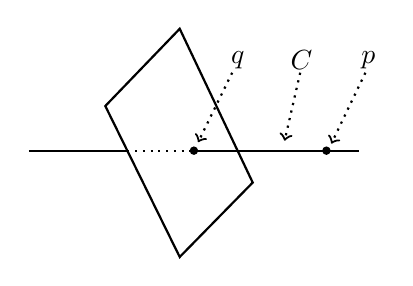
\begin{tikzpicture}[scale=0.9,line width=0.8pt]
  \draw (-0.2,1.72) -- (0.83,-0.45) -- (-0.2,-1.5) -- (-1.25,0.63) -- cycle;
  \draw (-2.33,0) -- (-0.94,0);
  \draw[dotted] (-0.94,0) -- (0,0);
  \draw (0,0) -- (2.33,0);
  \fill (0,0) circle (1.7pt);
  \fill (1.87,0) circle (1.7pt);
  \node at (0.62,1.28) {$q$};
  \draw[dotted,->] (0.54,1.1) -- (0.06,0.12);
  \node at (1.52,1.28) {$C$};
  \draw[dotted,->] (1.5,1.1) -- (1.28,0.14);
  \node at (2.46,1.28) {$p$};
  \draw[dotted,->] (2.42,1.1) -- (1.94,0.1);
\end{tikzpicture}
\caption{\trCodimension{}的行为。（依原书手绘图重绘。）}\label{fig:codim-behavior}
\end{figure}

\textbf{12.1.K.（容易的练习）}\quad 若 $Y$ 是\trScheme{} $X$ 的一个\trIrreducible{}\trClosedSubset，证明：
\begin{equation*}\tag{12.1.5.1}\label{eq:codim-dim-inequality}
\operatorname{codim}_X Y+\dim Y\le\dim X.
\end{equation*}
我们很快会看到：若 $X$ 与 $Y$ 都是\trIrreducible{}的\trVariety，则等号总成立（定理~12.2.9）；但等号在一般情形下并不成立（\S12.3.13）。

\emph{\trhWarning{}。}\ 「\trCodimension」这一观念仍可能表现得略微古怪。例如，考虑\cref{fig:codim-behavior}。（你应当把这幅图看作一幅直观示意图。）图中全空间 $X$ 的\trDimension{}为 $2$，而点 $p$ 的\trDimension{}为 $0$、\trCodimension{}为 $1$。我们还见到一个例子：\trCodimension{}为 $2$ 的子集 $q$ 含于\trCodimension{}为 $0$ 的子集 $C$，其间却没有「夹在中间」的\trCodimension{} $1$ 子集。

更糟的事情也可能发生；我们很快将在 \S12.3.13 中看到这样一个例子：\trIrreducible{}\trSurface{}中的一个\trClosedPoint{}，其\trCodimension{}是 $1$ 而非 $2$。然而，对\trIrreducible{}的\trVariety{}来说这种事不可能发生，并且不等式~\eqref{eq:codim-dim-inequality}必是等式（定理~12.2.9）。

\textbf{12.1.6. 在\trUFD{}中，\trCodimension{} $1$ 的诸\trPrimeIdeal{}都是\trPrincipalIdeal。}\quad 我们作一条简短的观察，以备日后引用。

\textbf{12.1.7.\ \trhLemma{}。}\ ——\ \emph{在\trUFD{} $A$ 中，诸\trCodimension{} $1$ 的\trPrimeIdeal{}都是\trPrincipalIdeal。}

这是「\trCodimension{} $1$ 相当特殊」这一事实的初次一瞥——这个主题将在 \S12.3 中延续。我们将会看到，\trhLemma{}~12.1.7 的逆命题也同样成立（当 $A$ 是\trNoetherian{}\trIntegralDomain{}时，见命题~12.3.7）。

\emph{证明。}\ 设 $\mathfrak{p}$ 是一个\trCodimension{} $1$ 的\trPrimeIdeal。任取 $\mathfrak{p}$ 中一个 $f\neq0$，并令 $g$ 是 $f$ 的落在 $\mathfrak{p}$ 中的任意一个不可约／素因子（这样的因子至少有一个）。于是 $(g)$ 是一个含于 $\mathfrak{p}$ 的非零\trPrimeIdeal，故 $(0)\subset(g)\subset\mathfrak{p}$。由于 $\mathfrak{p}$ 的\trCodimension{}为 $1$，必有 $\mathfrak{p}=(g)$，从而 $\mathfrak{p}$ 是\trPrincipalIdeal。\hfill$\square$

\textbf{12.1.8.\ \trDimension{}为 $0$ 的\trLocalRing。}\quad 维数为 $0$ 的对象并不只是些点；它们还携带着更进一步的信息，这些信息或可被想成某种无穷小的「形状」。稍早在 \S6.5 与\mbox{练习~8.3.G}中，我们已对这一点有过一瞥。

\textbf{12.1.9.\ 有用的\trhProposition{}。}\ ——\ \emph{设 $(A,\mathfrak{m})$ 是一个\trNoetherian\trLocalRing。那么下列诸条等价。}
\begin{enumerate}[label=(\roman*)]
\item $\dim A=0$；
\item $\mathfrak{m}=\mathfrak{N}(A)$；
\item 对某个 $n>1$，$\mathfrak{m}^n=0$；
\item $A$ 具有\trFiniteLength；
\item $A$ 中理想的任何降序列都最终恒定。
\end{enumerate}
\emph{这样的环称为\trArtin{}或\trFiniteLength{}局部环（定义~6.5.7）。}

\textbf{12.1.L.（练习）}\quad 证明\trhProposition{}~12.1.9。

\textbf{12.1.10.\ 一个有趣但不重要的反例。}\quad 我们以一个有趣的病理现象来为这个引导性的一节收尾。\trNoetherian{}环没有无穷的\trPrimeIdeal{}链，因此你也许会认为\trNoetherian{}环必定只有有限的\trDimension。\trNagata{}这位反例大师用下面的例子告诉你：事情并非如此。

\textbf{12.1.M.}\ \extrahard\ \textbf{（练习：一个无穷维的\trNoetherian{}环）}\quad 设 $A=k[x_1,x_2,\dots]$。取一个递增的正整数序列 $m_1,m_2,\dots$，使其差也递增（$m_{i+1}-m_i>m_i-m_{i-1}$）。令 $\mathfrak{p}_i=(x_{m_i+1},\dots,x_{m_{i+1}})$，并令 $S=A\setminus\bigcup_i\mathfrak{p}_i$。
\begin{enumerate}[label=(\alph*)]
\item 证明：$S$ 是一个\trMultiplicativeSubset。
\item 证明：$S^{-1}A$ 中的 $S^{-1}\mathfrak{p}_i$ 是某条长度为 $m_{i+1}-m_i$ 的\trPrimeIdeal{}链中最大的\trPrimeIdeal。从而得出结论：$\dim S^{-1}A=\infty$。
\item 设 $B$ 是一个满足如下两条的\trRing：(i) 对每个\trMaximalIdeal{} $\mathfrak{m}$，$B_{\mathfrak{m}}$ 都是\trNoetherian{}的；(ii) 每个非零的 $b\in B$ 都仅含于有限多个\trMaximalIdeal{}之中。证明：$B$ 是\trNoetherian{}的。（一种可能的进路：证明对任意的 $x_1,x_2,\dots$，$(x_1,x_2,\dots)$ 是\trFinitelyGenerated{}的。）
\item 用 (c) 证明：$S^{-1}A$ 是\trNoetherian{}的。
\end{enumerate}

\textbf{12.1.11.}\ \emph{\trhRemark{}：\trNoetherian\trLocalRing{}的\trDimension{}有限。}\quad 不过，我们将在\mbox{练习~12.3.K(a)}中看到：\trNoetherian{}局部环总是只有有限的\trDimension。（这需要一条出奇困难的事实——\trKrull{}高度定理~12.3.10。）因此，\trLocally\trNoetherian{}概形的点总具有有限的\trCodimension。
